\documentclass[main.tex]{subfiles} % Subfile-Class


% ============================================================================== %
%                            Subfile document                                    %
% ============================================================================== %

\begin{document}

% Template

\subsubsection{Strecken Rückverfolgung}

Dieser Abschnitt befasst sich damit, wie der Pfadfinder seinen Weg, den er
durch das Wegenetz genommen hat zurückverfolgen kann und so auf seine Position
Rückschliessen kann.

% ===================================================================================
\paragraph{Anforderungen}
Der Algorithmus setzt vorraus, dass das Gerät immer und zu jeder Zeit seine
Orientierung als absoluten Winkel ab dem Startpunkt weiss und die
zurückgelegten Strecken messen kann.

% ===================================================================================
\paragraph{Konzeption Wineklerfassung}
Betreffend dem Winkel könnte angenommen werden, dass ein einfacher Kompass auf
dem Gerät bereits ausreichen würde, um die Orientierung festellen zu können. Da
sich allerdings Motoren in der direkten Umgebung der Elektronik befindet,
welche ebenfalls starke Magnetfeldänderungen verursachen, bestehen zu grosse
Bedenken, dass der Winkel so eine willkürliche Form annimmt.

Anstelle dessen wird der Ansatz verfolgt, die momentane Änderungsrate des
Winkels über ein Gyroskop zu erfassen und in einem ausreichend geringen
Zeitintervall numerisch auf zu integrieren. Für die ersten Versuche dieses
Verfahrens wird ein einfaches Gyroskop des Typs \textit{MPU6050} eingesetzt,
welches viele Einstellmöglichkeiten im Sinne von Samplingraten und eines
integrierten Tiefpassfilters besitzt. Ausgelesen werden kann dieser über ein
einfaches $I^2C$ Protokoll. Abbildung~\ref{fig:MPU6050} zeigt eben dieses
Gyroskop als Evaluation Board - welches auf einem Steckbrett zu Testzwecken
eingesetzt wird.

\begin{figure}[h!]
    \centering
    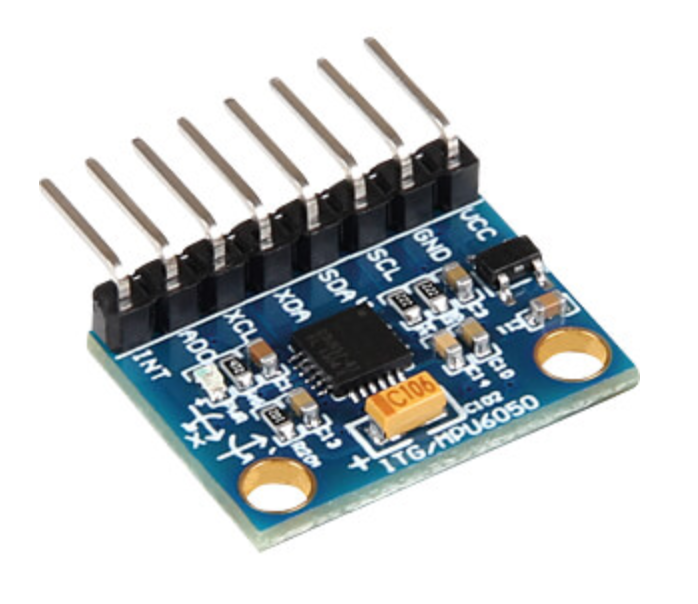
\includegraphics[width=1\textwidth]{./fig_Strecken_Tracken/MPU6050.png}
    \caption{MPU6050 Gyroskop EVAL-Board}~\label{fig:MPU6050}
\end{figure}

\paragraph{Konzeption Streckenerfassung}
Zur Rückverfolgung der zurückgelegten Strecke bieten sich gleich mehrere
Möglichkeiten. Der eingesetzte Schrittmotorentreiber wird nicht direkt über ein
Step/Dir Interface angesteuert, bietet allerdings trotzdem die Möglichkeit,
zurückgelegte Schritte via $SPI$ auszulesen. Da dies erst ausgiebig getestet
werden kann, wenn der Roboter ein erstes mal zusammengebaut wurde, werden
vorerst noch separate Encoder vorgesehen. Diese sind sehr einfach umgesetzt
anhand einer Lichtschranke, welche eine ausreichend gelochte Lochscheibe
auszählt.

==================================================
Text Yannik Dimensionierung Lochscheibe
==================================================

Entsprechende Signale auf dem Mikroprozessor erzeugen Interrupts, mit welchen
die Anzahl der Pulse dann ausgezählt werden. Grundsätzlich wird, wie im Kapitel
für Antriebe bereits erwähnt, der Antrieb nicht über Encoder geregelt sondern
über den Liniensensor. Daher wäre es naheliegend, dass der Raspberry-Pi diese
Encoder auszählt, da auch nur er auf diese Informationen zugreifen muss. Es ist
allerdings nicht sicher, wie gut der Raspberry Pi mangels Echtzeitfähigkeit
dafür geeignet ist, weshalb sich Encoder-Schnittstellen sowohl auf dem
Antriebscontroller als auch auf dem Raspberry-HAT befinden.

% ===================================================================================
\paragraph{Versuche Wineklerfassung}
Bei versuchen wurde mit verschiedenen Prarametern variiert, um ein gutes
Ergebnis zu erreichen. Die folgenden Parameter liefern ein sehr
zufriedenstellendes Ergebnis:

\begin{table}[h]                                    % h = here
    \centering
    \begin{tabular}{|c|c|}                        % c=centered, l=left, r=right
        \hline
        Parameter                         & Wert         \\ \hline
        Abfragehäufigkeit Mikrocontroller & $25 \mu s$   \\ \hline
        Samplingrate MPU6050              & $1 kHz$      \\ \hline
        Digital Low Pass Filter (DLPF)    & $f_g = 42Hz$ \\ \hline
    \end{tabular}
    \caption{Initialisierungsparameter MPU6050}
    \label{tab:params_mpu6050}
\end{table}

Per Software ist noch ein Treshhold-Wert eingestellt, mit welchem ganz leichtes
Zittern des Sensorwertes ignoriert werden kann. Mit diesen Werten können
Winkeländerungen von 360° in weniger als einer Sekunde problemlos erfasst
werden, ohne dass der Winkel in der Summe davon driftet. Diese Technik hat sich
also bewährt und wird auch so im Pfadfinder eingesetzt.

% ===================================================================================
\paragraph{Entscheidung und Fazit}
Fazit und Entscheid

\end{document}
